\documentclass{../../text-style}

\texttitle{Визуальное моделирование, UML}

\begin{document}

\maketitle
\thispagestyle{empty}

\section{Введение}

Как известно, при разработке ПО много времени требуется на анализ и проектирование. Если просто сесть и начать писать код, ничего хорошего из этого не выйдет. Для реализации программ есть удобные формализмы --- различные языки программирования, методологии и технологии. Для анализа и проектирования языки программирования, как правило, не годятся, поскольку требуют слишком детального изложения решения задачи. Там применяются свои специальные методики, например, при разработке алгоритмов --- псевдокод или блок-схемы. Блок-схемы на самом деле не используются уже давно, и по ходу дальнейшего изложения вы поймёте, почему.

Подавляющее большинство разрабатываемых приложений гораздо сложнее просто реализации алгоритма, поэтому нужно уметь выделять наиболее существенную информацию об архитектуре системы. Такое представление существенной информации без деталей реализации и называется моделью системы. Наиболее удобными и наглядными являются визуальные модели, где информация об архитектуре системы представляется в виде диаграмм. Наиболее близким аналогом визуальных моделей ПО в <<обычной>> инженерии являются чертежи --- так же, как здание строится по нарисованным архитектором чертежам, так и крупные приложения программируются по нарисованным архитектором визуальным моделям. Кроме того, визуальные модели применяются не только при проектировании, но и при общении между программистами --- гораздо проще показать картинку, по которой всё понятно, чем кучу кода, и при общении с заказчиком --- заказчик вообще программировать может не уметь, а если показать картинку, ему после краткого объяснения нотации всё сразу станет понятно. Ну и по тем же причинам диаграммы --- хорошее средство для документации. Ещё есть мнение, что диаграммы должны быть такими, чтобы по ним можно было сгенерировать исполняемый код --- не пропадать же уже нарисованным диаграммам. Это спорно, потому что для генерации кода диаграммы должны содержать все необходимые детали, что противоречит самой сути моделирования --- упрощению системы. Модель всегда должна быть проще того, что она моделирует, иначе в ней нет никакого смысла. Впрочем, программирование диаграммами (или визуальное программирование) вполне имеет право на жизнь и даже местами применяется, но слово <<моделирование>> при таком подходе неуместно.

Визуальные модели и чертежи имеют одно принципиальное отличие, вытекающее из принципиального отличия объектов физического мира и программ --- программное обеспечение невидимо. Здание, деталь, подводную лодку можно нарисовать, так, как мы увидим её глазами (или похоже), программное обеспечение мы не видим. Мы видим текст программы, видим внешние проявления работы программы, но это не сама программа. Как выглядит программа, вообще говоря, непонятно. Поэтому рисовать программные системы можно весьма по-разному. Поэтому любая визуализация программного обеспечения представляет собой некоторую метафору --- некоторые абстрактные и невидимые сущности программной системы сопоставляются видимым человеческому глазу объектам, всяким квадратикам и кружочкам. В общем-то, точно так же, эти абстрактные сущности сопоставляются тексту на конкретном языке программирования, или даже словесному описанию --- это лишь разные способы передать информацию об одном объекте. Из этих соображений, и ещё из того, что модель должна представлять только существенную информацию, следует ещё одно важное для визуального моделирования понятие: точка зрения моделирования. Визуальная модель всегда направлена на конкретную группу читателей, и служит конкретно для чего-то, не бывает просто визуальных моделей. Визуальные модели бывают трёх типов --- одноразовые, служащие исключительно для коммуникации, нарисовали диаграмму, потыкали в неё пальцами, изложили мысль и выкинули, документация --- такая модель, которую можно положить в гит или даже повесить на стенку (последний вариант бывает полезен при разработке больших систем, вешаем на стенку диаграмму с высокоуровневой архитектурой системы и стараемся ей следовать при разработке и сопровождении), и диаграммы, по которым генерируется код, фактически, графические исходники. Когда вы рисуете диаграмму, вы должны чётко понимать, зачем вы её рисуете. Если вы хотите объяснить кому-то идею решения задачи, вы рисуете только то, что существенно для объяснения, причём для объяснения именно того, что вы хотите объяснить, и именно тому, кому вы объясняете (картинки для директора и для вашего коллеги-программиста могут быть совсем разные).

Например, положим, есть задача сделать хеш-таблицу, но не простую, а так, чтобы хеш-функции туда можно было подставлять и менять по ходу работы (и, положим, мы это должны сделать на какой-нибудь старой версии C\#, где нет лямбда-функций). Можно было бы долго объяснять, что мы хотим отдельно интерфейс для хеш-функций, несколько его реализаций, и методы в хеш-таблице, которые бы принимали объекты этого интерфейса, но всё равно было бы непонятно. А можно просто нарисовать такую модель:

\begin{center}
    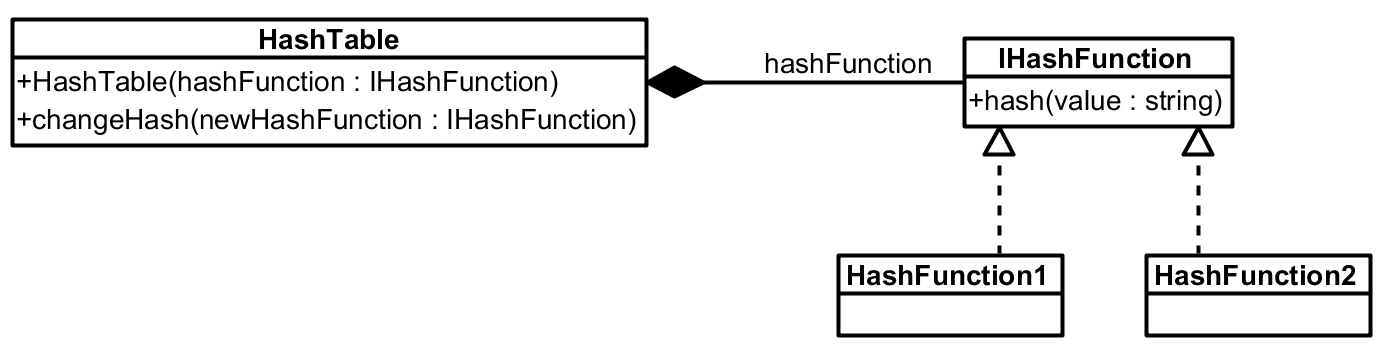
\includegraphics[width=0.9\textwidth]{modelExample.png}
\end{center}

Понятно, что у хеш-таблицы ещё куча методов, что она содержит ещё массив списков и всё такое, но к делу это имеет слабое отношение, а идея решения по этой диаграмме более-менее понятна: мы заводим интерфейс для хеш-функции, реализуем его в классах --- настоящих хеш-функциях, и передаём объекты этих классов конструктору хеш-таблицы, или специальному методу смены хеш-функции.

Понятно, что если рисовать диаграммы уж совсем абы как, от них будет мало пользы в деле передачи информации, потому что у каждого свои представления о том, как выглядит ПО. Требуется некая общепризнанная унифицированная нотация, чтобы незнакомые люди могли обмениваться диаграммами и однозначно понимать, что именно нарисовано. Такой нотации до 1996 года не было, была куча конкурирующих визуальных нотаций. В 1996 году авторов трёх наиболее популярных из них собрали вместе и велели ругаться, пока они не выработают единую нотацию. В результате они смогли договориться, так появился язык визуального моделирования UML. Та диаграмма, которая показана выше --- это пример диаграммы классов UML. Язык UML описывает довольно большое количество различных видов диаграмм (сейчас 13 штук), которые служат для описания программной системы с различных точек зрения --- высокоуровневая структура системы (из каких компонентов она состоит), более низкоуровневая структура (из каких классов состоит система и как эти классы взаимосвязаны), поведение системы, что делает система, как система располагается на физическом оборудовании, как организован обмен сообщениями в различных частях системы, как меняется состояние частей системы в зависимости от времени, и т.д. Диаграммы в UML делятся на две группы --- структуры (описывающие статическую структуру программы) и поведения (описывающие различные аспекты поведения системы во время выполнения). Вот диаграмма, показывающая отношения между диаграммами UML:

\begin{center}
    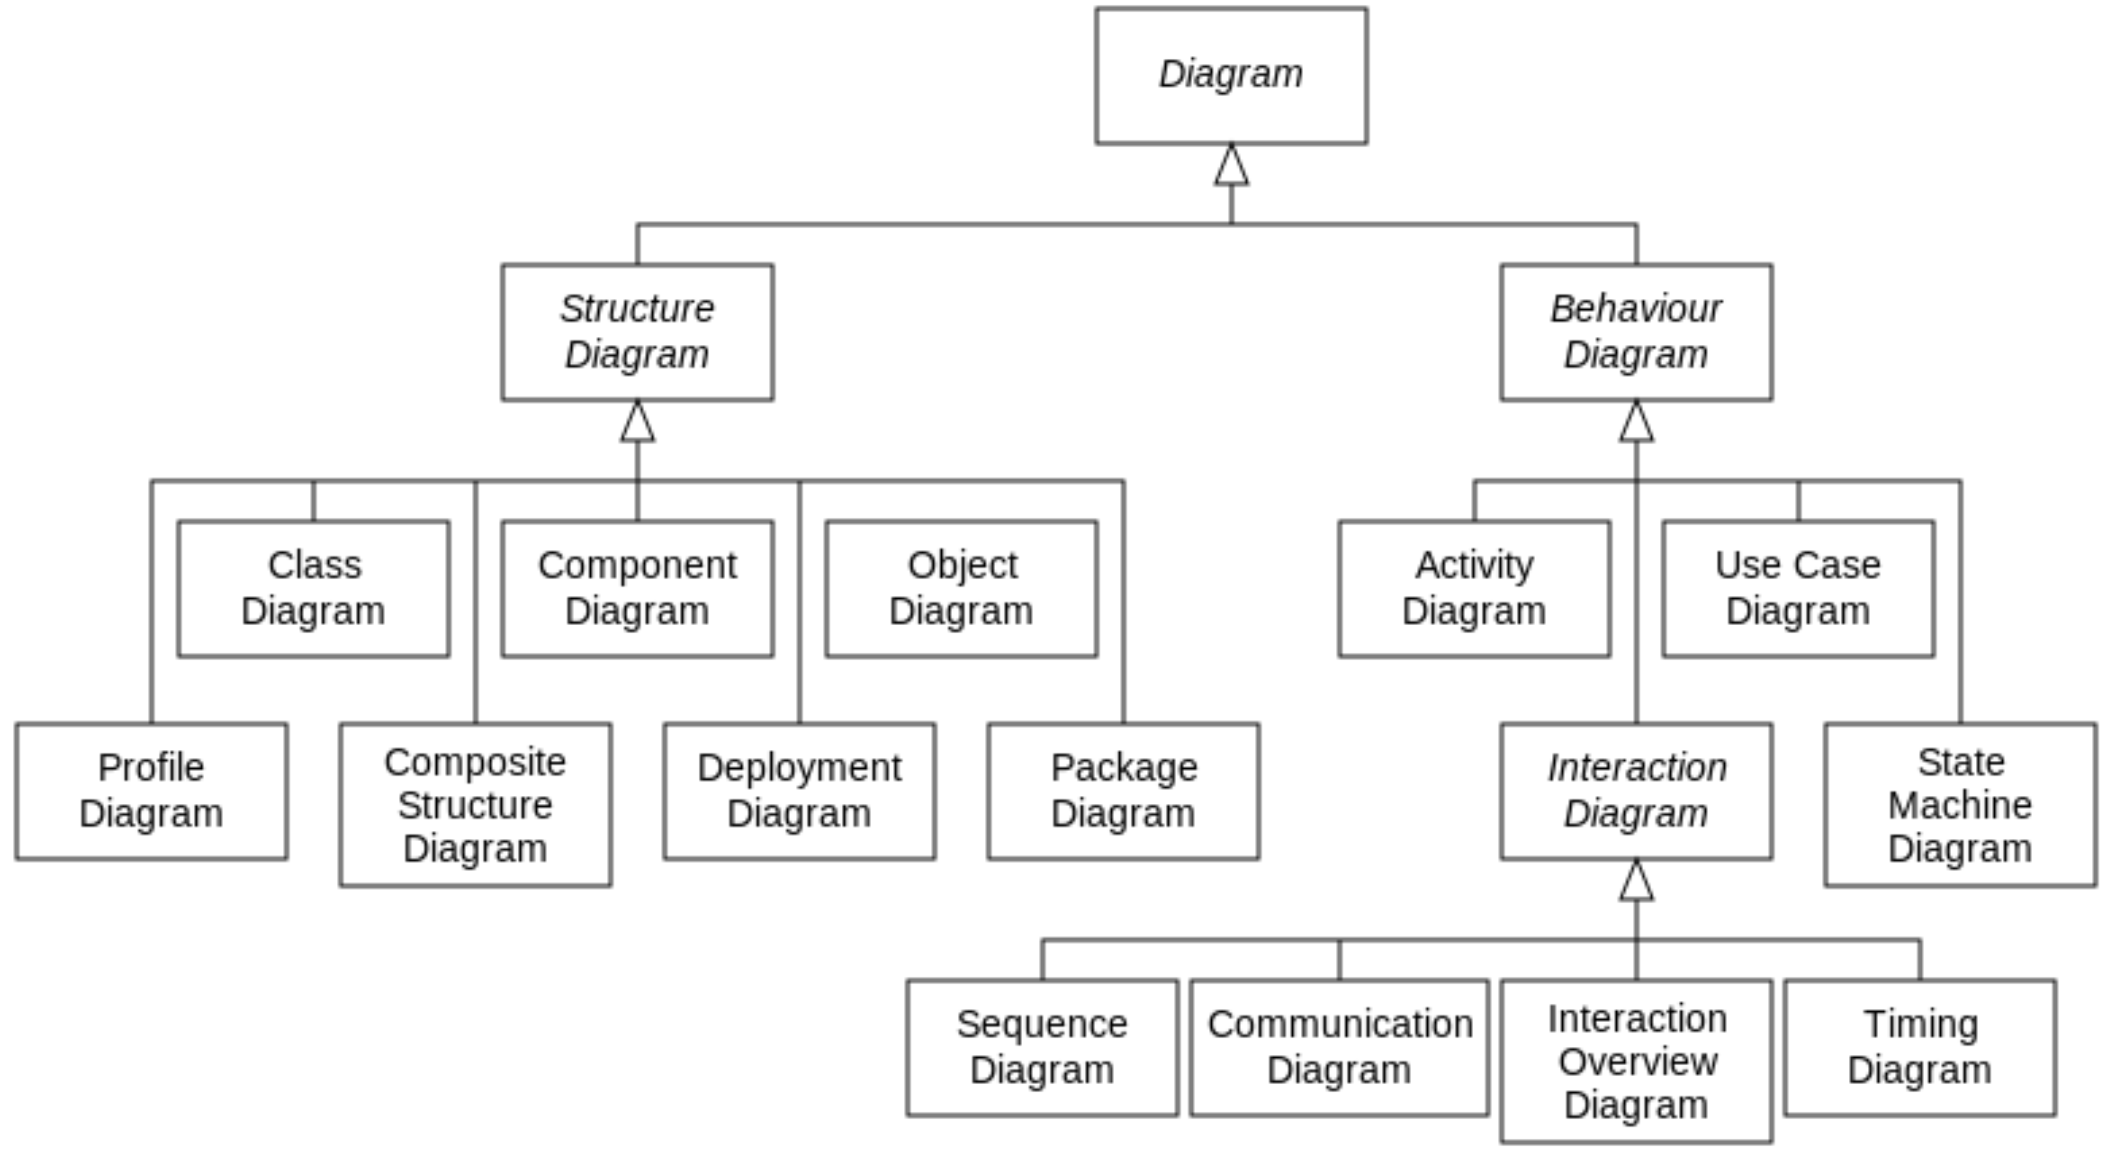
\includegraphics[width=0.9\textwidth]{umlDiagrams.png}
\end{center}

\section{Диаграммы классов}

Самая широко применяемая диаграмма UML --- это диаграмма классов. Диаграмма классов описывает типы объектов системы и различного рода статические отношения между ними. Там рисуются классы с полями и методами, и связи, которые могут быть между объектами этих классов. Вот картинка с синтаксисом диаграммы:

\begin{center}
    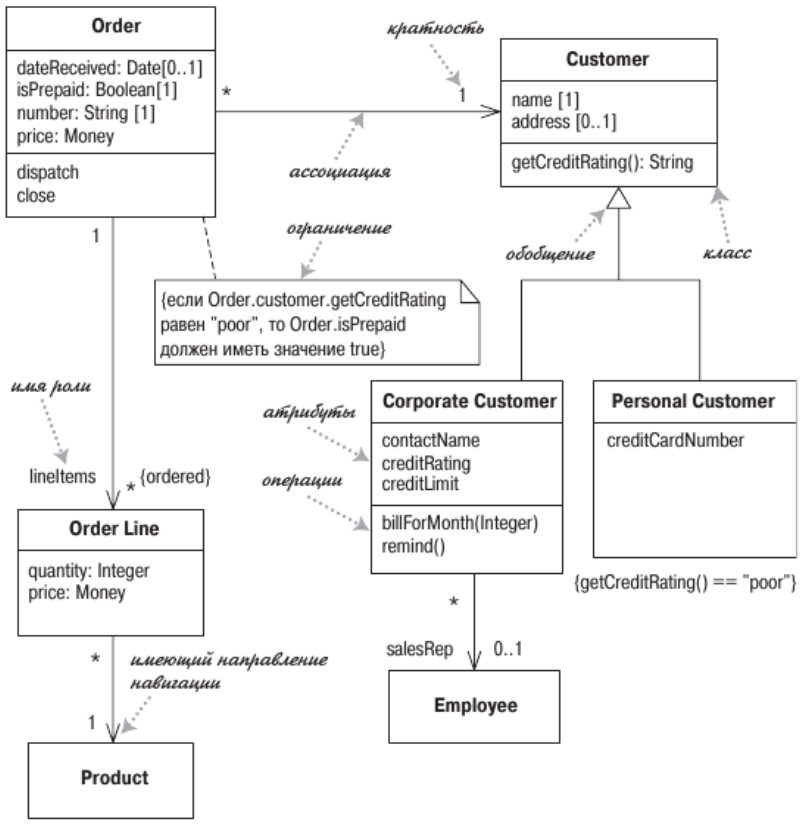
\includegraphics[width=0.7\textwidth]{umlClassDiagram.png}
\end{center}

В общем случае объявление поля выглядит как <<видимость имя: тип кратность = значение по умолчанию {строка свойств}>>. Обязательно только имя. Видимость бывает + (public), - (private), \# (protected), \textasciitilde (package). Кратность может задаваться в виде 1 (ровно 1 объект), 0..1 (ни одного или один), * (сколько угодно), можно 1..*, можно 2..*. Поле не обязательно описывать как, собственно, поле, его можно изобразить в виде ассоциации, как показано на картинке выше, например, у товара может быть несколько строк заказа, тогда как каждой строке заказа соответствует один товар. Ассоциации могут иметь направление (направление навигации), показывающее, какой класс о каком знает, ассоциация может быть двунаправленной, если направление не задано, то либо ассоциация двунаправленная, либо направление на данном уровне моделирования просто не важно. Статические поля и методы рисуются подчёркнутыми.

Ещё можно явно указать тип ассоциации:

\begin{center}
    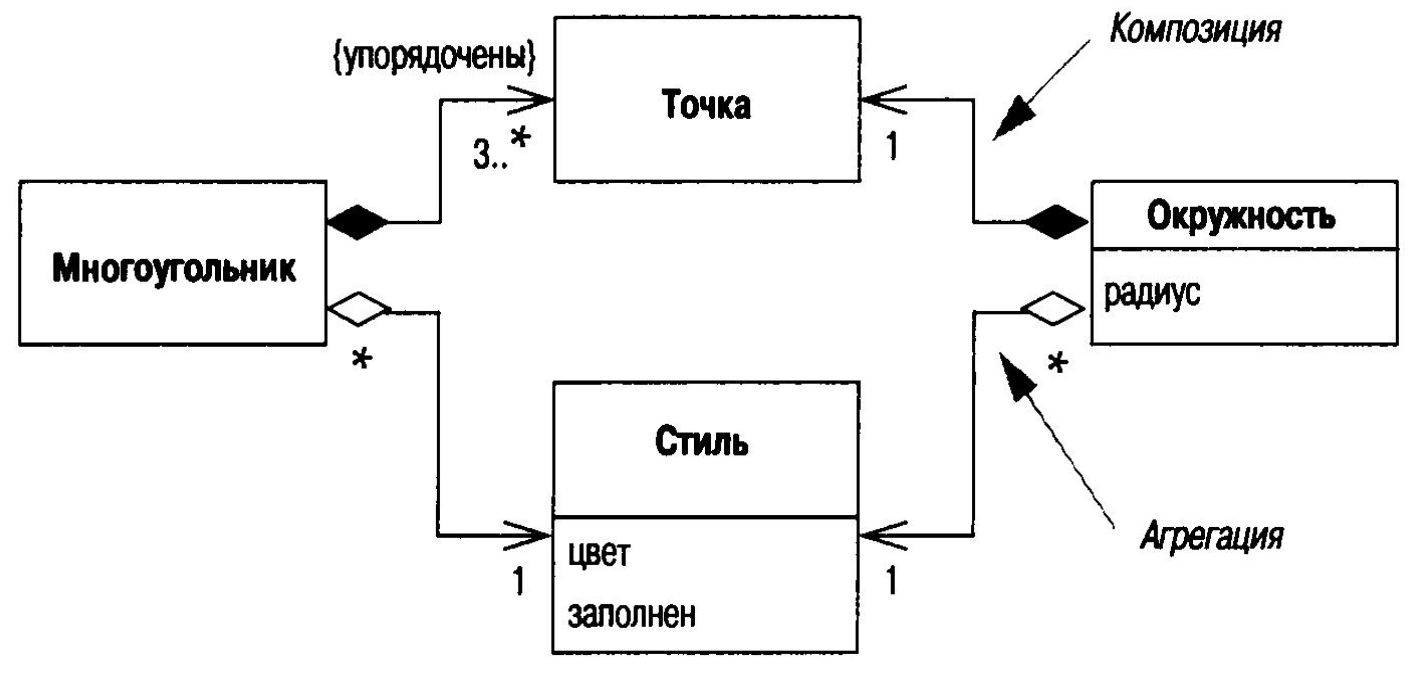
\includegraphics[width=0.6\textwidth]{associationTypes.png}
\end{center}

Бывают ассоциации агрегации и композиции. Агрегация, как правило, это отношение, показывающее, что один объект знает о другом и может инициировать с ним взаимодействие. Композиция задаёт отношение владения --- экземпляр класса, участвующего в композиции, может иметь только одного объекта-владельца, несмотря на то, что сам класс может участвовать в нескольких отношениях композиции. Агрегация же говорит, что класс просто знает о другом классе, но не владеет им. Например, на картинке точка может быть либо вершиной многоугольника, либо центром окружности, но не и тем и другим одновременно. Тогда как стиль для всех объектов может быть один. Важно помнить, что объекты,  связанные отношением композиции с объектом-владельцем, не могут жить отдельно от него, так что когда его удаляют, они удаляются вместе с ним. Поэтому отношение композиции показывает свойства, которыми владеют по значению (это весьма важно для С++ и не так существенно для C\# или Java --- в C\# и Java есть сборка мусора, а вот в С++ ясное понимание отношений владения нужно для управления памятью). Агрегация и композиция являются частными случаями ассоциации, так что допустимо на более высокоуровневых диаграммах рисовать их как просто ассоциации, а когда это становится важным (ближе к реализации) --- специфицировать, что именно за ассоциацию мы имеем в виду.

Интерфейсы и абстрактные классы рисуются вот так:

\begin{center}
    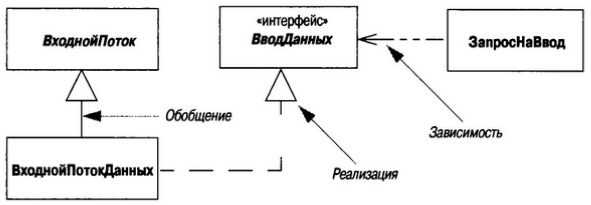
\includegraphics[width=0.7\textwidth]{interfaces1.png}
\end{center}

Имена абстрактных классов пишутся курсивом, интерфейсов --- тоже, но ещё и с <<interface>>. Реализация и зависимость (то есть использование интерфейса) --- на картинке понятно как. Обобщение ещё называют генерализацией, это отношение наследования. Можно рисовать интерфейсы ещё и так:

\begin{center}
    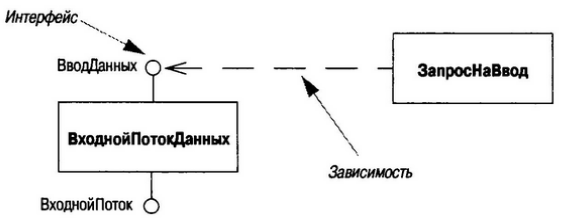
\includegraphics[width=0.6\textwidth]{interfaces2.png}
\end{center}

Такая нотация обычно применяется для достаточно крупных частей системы, например, для компонентов.

Можно даже генерики рисовать:

\begin{center}
    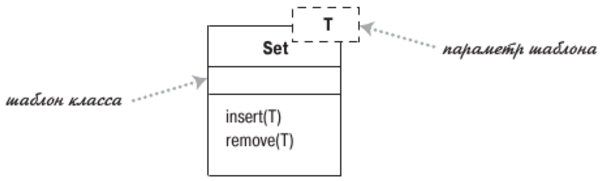
\includegraphics[width=0.7\textwidth]{templates.png}
\end{center}

Комментарии рисуются так:

\begin{center}
    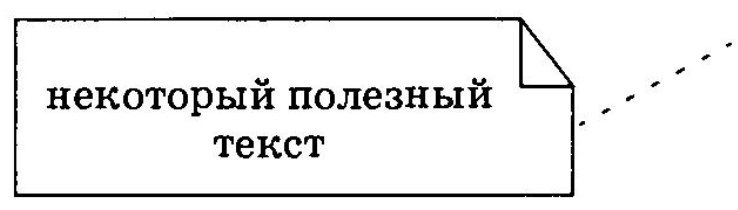
\includegraphics[width=0.4\textwidth]{comment.png}
\end{center}

Цепляются пунктирной линией к тому, что они комментируют. Комментарии можно рисовать не только на диаграмме классов, но и где угодно. Можно их ни с чем не связывать, тогда это будет комментарий к диаграмме вообще.

\section{Диаграммы компонентов}

К диаграммам, которые можно нарисовать и повесить на стенку, относятся, в частности, диаграммы компонентов. Диаграммы компонентов показывают различные компоненты системы и связи между ними. Что такое компонент --- вопрос сложный, о котором до сих пор спорят, но вполне можно считать компонент просто большой и обособленной частью системы (обособленность здесь, пожалуй, ключевое свойство). Компоненты полезно использовать вместе с диаграммами размещения (да, UML допускает смешивать нотации разных видов диаграмм, но надо использовать это осторожно). Выглядит это как-то так:

\begin{center}
    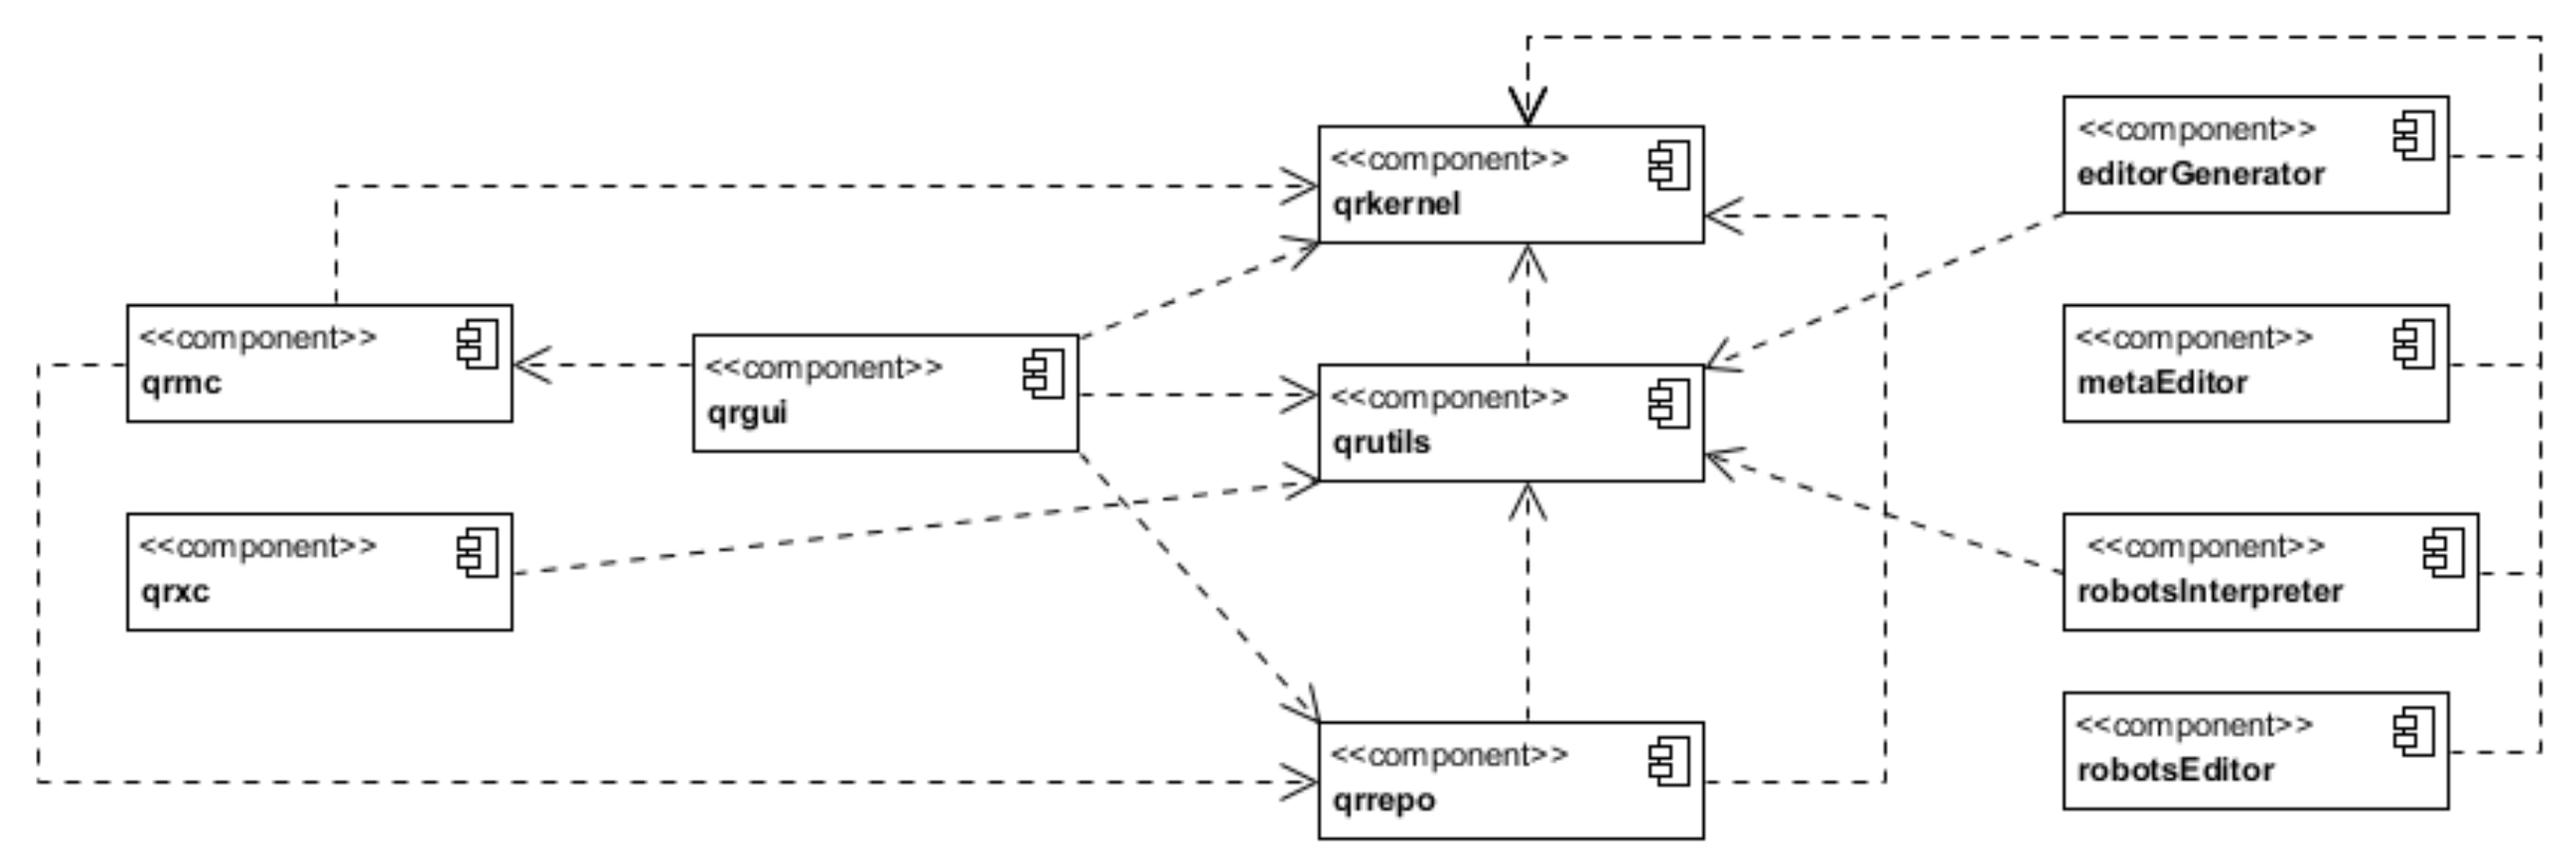
\includegraphics[width=0.95\textwidth]{componentDiagram.png}
\end{center}

Компоненты раньше использовались для представления физических частей системы --- .dll, например. Теперь для этого используется другая нотация, так что можно использовать диаграммы компонентов для рисования высокоуровневой архитектуры системы. Это, пожалуй, самые полезные для архитектора диаграммы, и с них по идее стоит начинать архитектурное описание своего проекта (которое вам придётся писать на втором курсе).

Вот описание синтаксиса диаграмм компонент, на сей раз с сайта \url{http://www.uml-diagrams.org} (очень рекомендую, как быструю справку по синтаксису и как набор примеров с пояснениями):

\begin{center}
    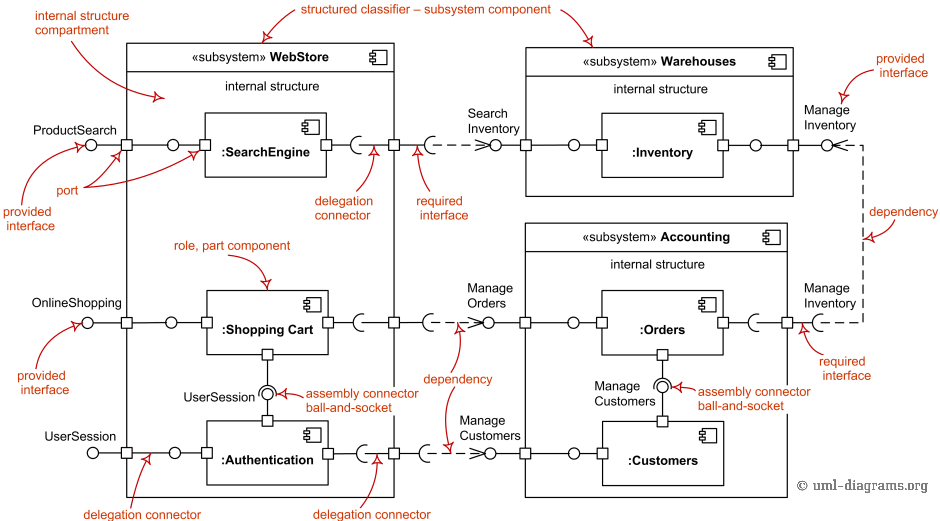
\includegraphics[width=0.95\textwidth]{componentDiagramsOverview.png}
    \attribution{\url{http://www.uml-diagrams.org}}
\end{center}

Видно, что компоненты могут быть вложенными друг в друга, что они могут иметь интерфейсы (так же, как и классы, но на диаграммах компонентов чаще всего используется только <<леденцовая>> нотация). У компонентов есть порты, которые могут предоставлять или потреблять интерфейсы, но порты часто не рисуются, а подразумеваются, поскольку обычно порт имеет только один интерфейс. Порты бывают полезны для изображения делегирования --- что компонент просто перенаправляет запросы вложенному компоненту. Слова \verb|<<subsystem>>| и <<internal structure>> опциональны (и обычно не пишутся).

\section{Диаграммы случаев использования}

Ещё одной часто используемой и весьма полезной диаграммой UML является диаграмма случаев использования (или прецедентов, use case diagram). Используются они на фазе анализа для определения и обсуждения функциональных требований к системе. На диаграмме описываются типичные взаимодействия между пользователями системы и самой системой. Анализ требований к системе обычно начинается с описания сценариев взаимодействия пользователя и системы. Например, делаем мы онлайн-магазин. Неплохо бы, чтобы там было можно купить товар. Опишем, как происходит покупка товара: <<Покупатель просматривает каталог и помещает выбранные товары в корзину. При желании оплатить покупку он вводит информацию о кредитной карте и производит платёж. Система проверяет авторизацию кредитной карты и подтверждает оплату товара тотчас же и по электронной почте>>. Это один сценарий, если у нас есть постоянный клиент, для которого проверка информации о кредитной карте необязательна, появится другой сценарий. В любом случае, цель у пользователя одна --- купить товар. Вот множество сценариев, объединённое общей целью и называется случаем использования. В терминах UML пользователи называются актёрами (actor). Актёр представляет не конкретного пользователя, а роль, которую пользователь играет по отношению к системе --- один и тот же человек может выступать в двух ролях (например, админ онлайн-магазина сам может делать в нём покупки). Заметьте, что в роли актёра может выступать не только человек, но и другая система, внешняя по отношению к нашей, или другой компонент системы, если мы рисуем диаграмму случаев использования для компонента. 

Выглядит диаграмма так:

\begin{center}
    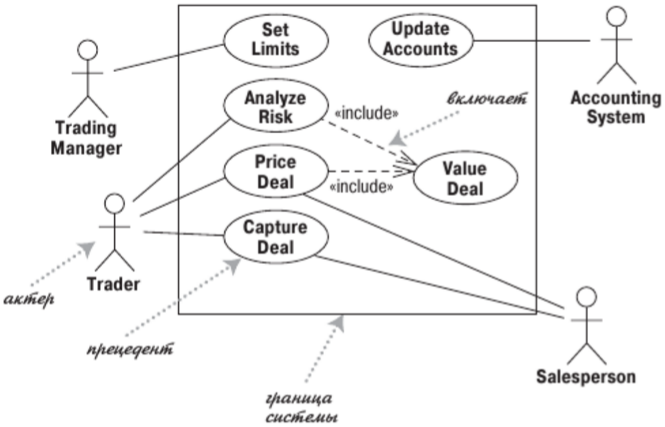
\includegraphics[width=0.7\textwidth]{useCaseDiagram.png}
\end{center}

Между случаями использования могут быть отношения обобщения (на самом деле, между актёрами тоже), отношения включения. Однако, умные люди рекомендуют не заморачиваться, а сконцентрировать внимание на текстовом описании случаев использования --- которое должно включать типичный сценарий взаимодействия в этом случае использования и возможные отклонения от этого сценария. С такой диаграммой и текстовыми описаниями вы будете чётко представлять, что вы хотите от системы. Например, для написания калькуляторов такое бы весьма сгодилось --- непродуманное поведение при нажатии на знаки арифметических операций приводило к забавным багам.

\section{Диаграммы активностей}

Следующая весьма распространённая диаграмма --- это диаграмма активностей (или диаграммы деятельности). Они служат для описания поведения системы. То есть, на самом деле, их предназначение --- моделирование бизнес-процессов и потоков работ, но они вполне могут использоваться и для описания поведения методов. Выглядят они вот так:

\begin{center}
    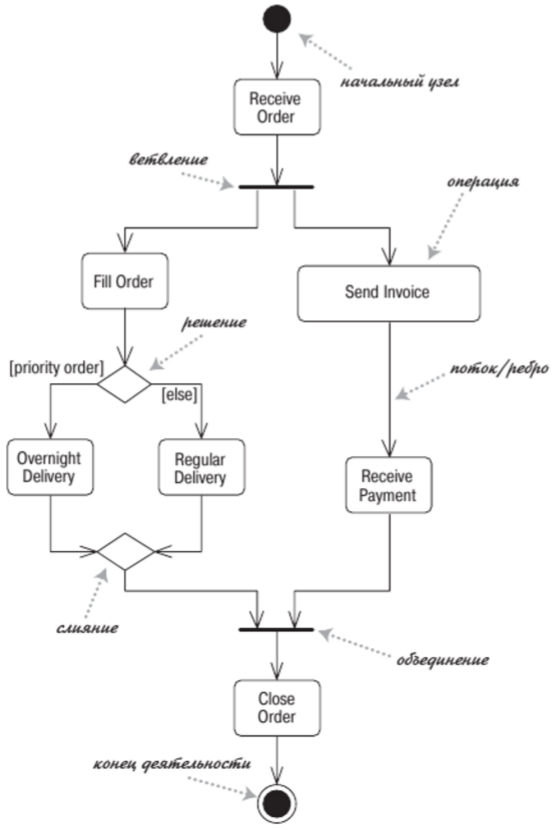
\includegraphics[width=0.7\textwidth]{activityDiagram.png}
\end{center}

 - очень похоже на блок-схему, однако же, имеет нотацию для параллельного исполнения и другие вещи, которых в классических блок-схемах нет. Обычно такими диаграммами моделируются процессы, происходящие в реальном мире, где в итоге должна будет работать создаваемая система, для лучшего понимания её окружения. Ещё такими диаграммами можно описывать высокоуровневое поведение системы --- что именно она делает и в какой последовательности. Ещё можно такими диаграммами специфицировать реализацию каждого конкретного метода каждого класса, составляющего систему, но толку от таких диаграмм мало, потому что код в текстовом виде вполне может оказаться понятнее (такие диаграммы имеют свойство быстро расти в размерах и сложности). Действия на диаграмме могут сами раскрываться в поддиаграммы:

\begin{center}
    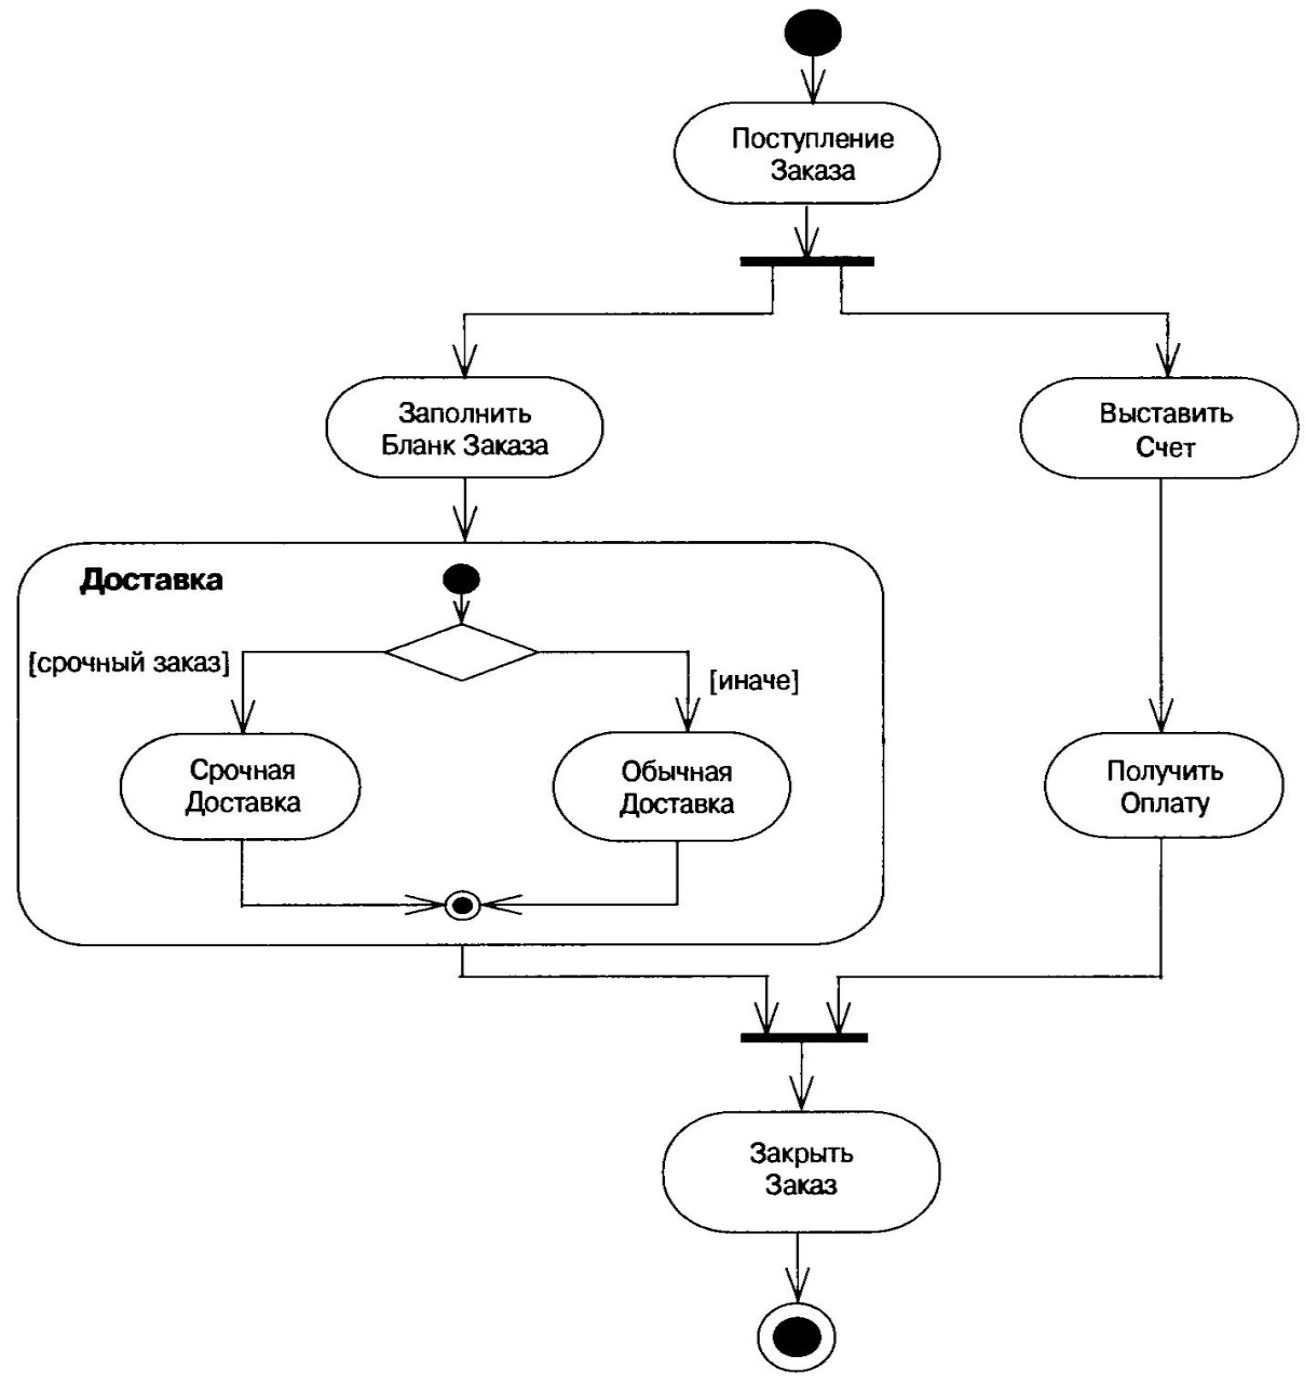
\includegraphics[width=0.7\textwidth]{activitySubdiagrams.png}
\end{center}

На этих диаграммах могут рисоваться ещё разные вещи, например, посылка и приём сигнала (но вам оно пока не нужно, потому что параллельные программы мы пока не писали), сигналы таймера, исключения, разделы (или дорожки), структурные узлы, задающие циклы, участки параллельного исполнения и т.д. Следует отметить, что диаграммы активностей --- одно из немногих мест в UML с более-менее чётко заданной семантикой, так что по таким диаграммам можно генерировать исполняемый код. Однако же, обычно для генерации кода и исполнения используются не диаграммы активностей, а диаграммы конечных автоматов.

\section{Диаграммы последовательностей}

Следующий тип диаграмм UML, использующийся при моделировании поведения --- это диаграммы последовательностей (sequence diagrams). Они применяются для визуализации взаимодействия между объектами --- передачи сообщений, возврата значений, времени жизни объекта. Выглядят диаграммы следующим образом:

\begin{center}
    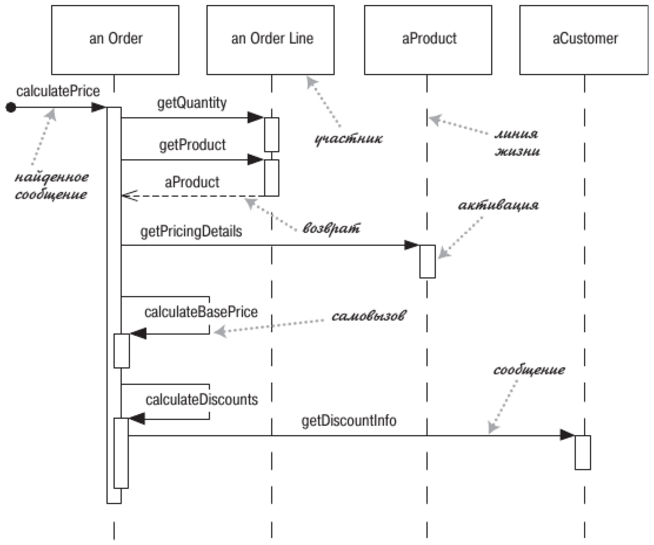
\includegraphics[width=0.8\textwidth]{sequenceDiagram.png}
    \attribution{М. Фаулер, UML. Основы}
\end{center}

На диаграмме рисуются объекты (обратите внимание, не классы), из каждого объекта выходит \textit{линия жизни} (пунктирная линия), на которой расположены \textit{линии активации} (длинный белый прямоугольник). Линия жизни показывает, когда объект вообще существует в памяти, линия активации --- когда объект занят какой-то работой (то есть работает либо его метод, либо метод, вызванный из его метода, или, более формально, какой-либо из методов объекта находится на стеке вызовов). Линий активации одновременно может быть несколько --- рекурсивные вызовы. Стрелки между линиями активации обозначают сообщения --- как правило, это вызовы методов, и поэтому они ведут в начало соответствующих вызванному методу линий активации. Обратите внимание, что стрелка не может выходить из неактивного объекта и не может входить <<в никуда>>.

Такая диаграмма позволяет разобраться в даже довольно сложных протоколах взаимодействия, поэтому применяется при многопоточном и асинхронном программировании, чтобы визуализировать общение между потоками/асинхронные вызовы. Также такие диаграммы очень популярны при описании телекоммуникационных протоколов (на самом деле, есть отдельный язык MSC (Message Sequence Charts), который применяется независимо от UML, но диаграммы последовательностей являются его почти копией).

\section{Диаграммы конечных автоматов}

Диаграммы конечных автоматов (или диаграммы состояний, state machine diagrams) служат для спецификации поведения классов, в отличие от диаграмм активностей, которые специфицируют поведение конкретного метода. На диаграмме изображаются все возможные состояния объекта, а также изменения состояния объекта, которые происходят вследствие влияния неких внешних событий на этот объект. Выглядит диаграмма так:

\begin{center}
    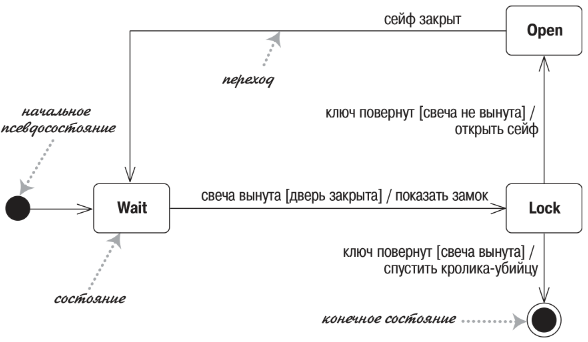
\includegraphics[width=0.7\textwidth]{stateTransitionSyntax.png}
\end{center}

На диаграмме изображены состояния (state) и переходы (transition). Переходы имеют метки, в формате <<триггер-идентификатор [защита]/активность>>, все они необязательны. Триггер-идентификатор указывает, по какому событию может происходить переход, защита --- логическое условие, которое должно быть выполнено, чтобы переход состоялся. Активность --- что надо делать во время перехода. Тут может быть ссылка на диаграмму активностей. Активности могут писаться и прямо внутри состояния (они называются внутренними активностями), синтаксис там такой же, а работают они как переходы из состояния в себя с выполнением нужной активности. Состояния могут быть вложенными, есть возможность указать параллельные состояния, но как --- выходит за рамки лекции.

Заметим, что диаграммами автоматов (хотя и менее общими) мы пользовались в первом семестре, когда писали лексические анализаторы. Ещё следует обратить внимание на отличие диаграмм автоматов и диаграмм активностей (хотя бы потому, что диаграммы активностей выделили в отдельный вид диаграмм не с первых версий UML). В диаграммах активностей действия выполняются в узлах, а в диаграммах автоматов --- при переходах. Кроме того, как уже говорилось, диаграммы автоматов рисуются для всего класса, а активностей --- для каждого конкретного метода. Диаграмма автоматов более высокоуровневая, чем диаграмма активностей, однако, с её помощью удобно реализовывать только системы, хорошо выражающиеся в терминах конечных автоматов (те же лексические анализаторы). Впрочем, в ИТМО есть большая группа уважаемых людей (во главе с проф. Шалыто), полагающая, что диаграммы автоматов способны адекватно описать вообще любую систему, и они умеют делать даже визуальные отладчики диаграмм автоматов. Другие не менее уважаемые люди (Фаулер, например), впрочем, считают, что диаграммы автоматов не годятся для описания сложных систем взаимодействующих объектов.

\subsection{Генерация кода}

Конечные автоматы хороши тем, что по ним можно легко и приятно генерировать код, в силу их стандартизованной семантики. Рассмотрим пример с кроликом-убийцей из книжки Фаулера:

\begin{center}
    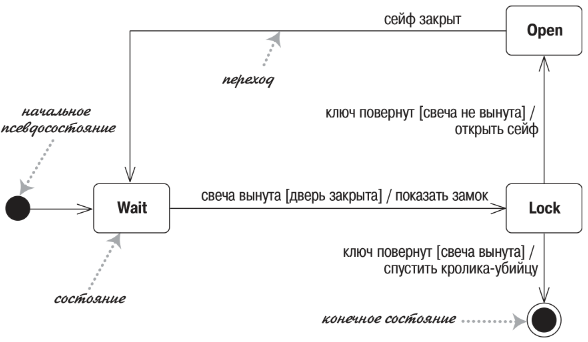
\includegraphics[width=0.8\textwidth]{stateTransitionSyntax.png}
    \attribution{М. Фаулер, UML. Основы}
\end{center}

Первый, самый простой способ сгенерировать код --- это сгенерировать гигантский switch, внутри которого чуть менее гигантские switch-и. Внешний switch --- по текущему состоянию автомата, внутренние --- по событиям, на которые находясь в данном состоянии автомат может реагировать. Внутри --- проверка условий стражников, выполнение действия по переходу и переход в следующее состояние. Состояние моделируется enum-ом, хранящимся как поле объекта. Для нашего примера получится что-то такое:

\begin{minted}{java}
public void handleEvent(PanelEvent anEvent) {
    switch (currentState) {
        case PanelState.Open:
            switch (anEvent) {
                case PanelEvent.SafeClosed:
                    currentState = PanelState.Wait;
            }
            break;
        case PanelState.Wait:
            switch (anEvent) {
                case PanelEvent.CandleRemoved:
                    if (isDoorOpen) {
                        revealLock();
                        currentState = PanelState.Lock;
                    }
            }
            break;
        case PanelState.Lock:
            switch (anEvent) {
                case PanelEvent.KeyTurned:
                    if (isCandleIn) {
                        openSafe();
                        currentState = PanelState.Open;
                    } else {
                        releaseKillerRabbit();
                        currentState = PanelState.Final;
                    }
            }
            break;
    }
}
\end{minted}

Это работает, но если этот код надо сопровождать, никто от него не будет в восторге. Для сколько-нибудь содержательных автоматов получается один метод на тысячи строк. Поэтому можно использовать таблицу состояний и универсальный интерпретатор, который просто ищет в таблице текущее состояние и событие, и выполняет то, что там написано. Вариантов таблиц состояний может быть много, но вот пример из книжки Фаулера:

\begin{center}
    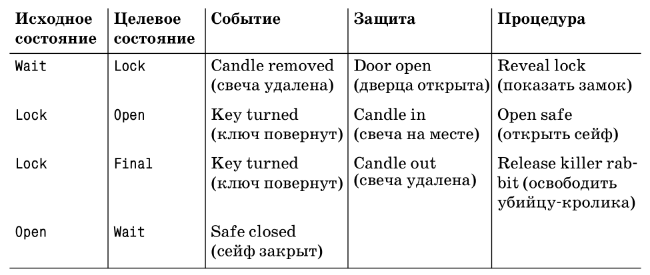
\includegraphics[width=0.6\textwidth]{stateTransitionStateTable.png}
    \attribution{М. Фаулер, UML. Основы}
\end{center}

Таблица состояний обычно либо хранится как файл данных рядом с программой, либо вкомпилируется в исходный код. 

Такой подход очень популярен в лексическом и синтаксическом анализе, но отлаживать или просто понимать такие программы очень тяжело. Поэтому есть ещё один, более объектно-ориентированный способ симулировать автомат: паттерн проектирования <<Состояние>>:

\begin{center}
    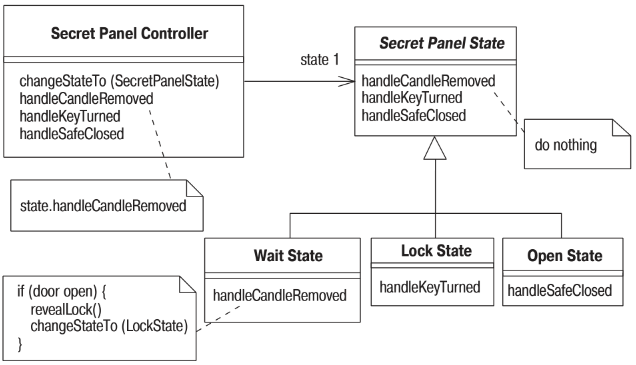
\includegraphics[width=0.6\textwidth]{stateTransitionStatePattern.png}
    \attribution{М. Фаулер, UML. Основы}
\end{center}

Автомат представляется в виде класса, который имеет в качестве поля ссылку на интерфейс <<текущее состояние>>. Этот интерфейс имеет столько методов, сколько всего разных событий может обрабатывать автомат. Интерфейс реализуют конкретные классы, отвечающие за конкретные состояния, они определяют те методы интерфейса, на которые могут реагировать, там уже проверяют условия стражников и выполняют действие при переходе. Каждый такой метод возвращает объект-состояние, в которое должен перейти автомат дальше. То есть, по сути, это тот же switch, где самый большой switch (по состояниям) спрятан в таблицу виртуальных методов. Такой подход делает реализацию автомата более-менее читаемой, ограничивает ответственность каждого класса только одним состоянием и позволяет очень легко добавить новые состояния, поэтому очень популярен при <<ручной>> реализации автоматов.

\section{Диаграмма развёртывания UML}

Диаграмма развёртывания UML (deployment diagram) используется для того, чтобы показать размещение логических элементов системы (компонентов, исполнимых файлов) на физических или виртуальных устройствах. Пример такой диаграммы:

\begin{center}
    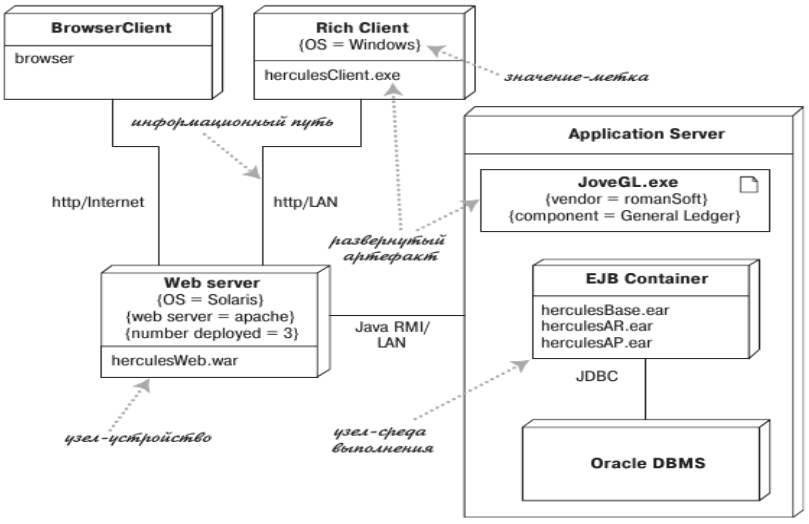
\includegraphics[width=0.7\textwidth]{deploymentDiagram.png}
    \attribution{М. Фаулер, UML. Основы}
\end{center}

Параллелепипедами на диаграмме рисуются устройства или похожие на устройства части системы (реальные компьютеры или группы компьютеров, базы данных, среды выполнения и т.д.). В них рисуются развёрнутые там артефакты (бинарники, компоненты и т.д.). Связи здесь возможны только между узлами (устройствами) и показывают они физические (или низкоуровневые логические) каналы связи между узлами, с указанием протокола взаимодействия. И узлы, и артефакты могут иметь дополнительные свойства, пишущиеся в фигурных скобках. Артефакты можно рисовать как подробно (прямоугольником), так и кратко (просто надписью с именем артефакта).

\section{CASE-инструменты}

Ещё один немаловажный вопрос, который осталось обсудить --- это а где рисовать эти все диаграммы. Существуют специальные программы для визуального моделирования, которые отличаются от графических редакторов тем, что <<понимают>>, что в них рисуют (и позволяют рисовать, например, класс UML, а не просто прямоугольник с текстом), и умеют довольно многое делать с диаграммами --- генерировать код, интерпретировать диаграммы, строить диаграммы по коду, искать антипаттерны и т.д. Такие программы называются CASE-инструментами (от Computer-Aided Software Engineering).

Существующие CASE-инструменты можно условно разделить три категории.

\begin{itemize}
    \item <<рисовалки>> --- не очень умные инструменты, которые позволяют удобно рисовать диаграммы и иногда немного генерить по ним код, но не пытаются помогать с архитектурой или отладкой программы. Используются прежде всего как графические редакторы, специально заточенные под рисование диаграмм. Иногда люди увлекаются и начинают хотеть от них большего (например, генерации исполнимого кода по модели в Visio), но для этого есть лучшие альтернативы. Примеры таких инструментов:
    \begin{itemize}
        \item Microsoft Visio --- часть пакета Microsoft Office, на самом деле редактор диаграмм вообще, UML там один из десятков разных вариантов (от диаграмм из кружочков и стрелочек до планов помещений). Причём, UML, хоть и есть в стандартной поставке, там не очень продвинутый (некоторых элементов нотации не хватает), так что лучше отдельно поставить плагин с полноценной поддержкой UML (благо в Visio есть развитая плагинная система). Visio очень популярен в бизнес-среде, но платный (и, кажется, даже не входит в студенческую подписку СПбГУ, хотя и есть в компьютерных классах), и работает только под Windows.
        \item Dia --- Visio для Linux. Как часто бывает в Linux, бесплатна, с открытым исходным кодом, есть в репозитории любого уважающего себя дистрибутива, имеет кучу плагинов (в том числе, поддержку UML), умеет генерировать код. Больше практически ничего не умеет, поэтому как настоящая CASE-система не используется.
        \item SmartDraw --- рисовалка диаграмм вообще, не только программистских. Работает под Windows и имеет веб-версию, но платная.
        \item LucidChart --- примерно то же самое, несколько менее платное в том смысле, что сколько-то простых диаграмм на одного пользователя можно рисовать бесплатно. Имеет только веб-версию (и вроде как мобильные версии) и очень агрессивную рекламу.
        \item Creately --- простая, но относительно удобная веб-рисовалка. Рисует страшные как моя жизнь диаграммы, но если надо быстро что-то нарисовать без установки и длительного процесса регистрации, Creately вполне подойдёт.
        \item draw.io (она же diagrams.net) --- несколько более крутая веб-рисовалка, интегрируется с Google Drive, рисует гораздо более симпатичные диаграммы, чем Creately, но может быть несколько менее удобной. Всенародно любима (студенты на курсе по архитектуре в основном ей пользуются).
    \end{itemize}
    \item Полноценные CASE-системы --- то самое, про что шла речь в предыдущем разделе. Как правило, платные, но, как правило, имеются бесплатные Community-версии, поэтому рекомендую пользоваться именно этими штуками, а не <<рисовалками>>. Как правило, все такие штуки десктопные, кроссплатформенные, с несколько урезанной браузерной версией. Популярные примеры:
    \begin{itemize}
        \item Enterprise Architect --- довольно популярный в IT-индустрии инструмент, более-менее всё умеет (не только UML, но и BPMN, SysML и другие полезные штуки) и не очень дорог (от 300\$ за лицензию и без бесплатной версии, так что для бедных студентов или инди-разработчиков так себе, но даже для средних стартапов это копейки).
        \item Rational Software Architect --- бывший Rational Rose (самый первый инструмент, поддерживавший UML), переписанный на платформе Eclipse. Тоже более-менее всё умеет, зато дороговат и опять-таки без бесплатной версии. Ни разу не видел, чтобы его использовали при практической разработке ПО, возможно это как-то связано с крайним неудобством его официального сайта. Достоин упоминания из-за отличной поддержки архитектурных рефакторингов.
        \item MagicDraw --- говорят, довольно хорошая и довольно популярная CASE-система, но, опять-таки, не видел её в деле.
        \item Visual Paradigm --- сам ей пользуюсь и встречал в индустрии, очень рекомендую. Умеет очень много чего, но основное её достоинство --- это usability. И наличие Community-версии.
        \item GenMyModel --- скорее, очень продвинутая браузерная <<рисовалка>>, чем настоящая CASE-система, но умеет генерировать код, умеет UML, BPMN и ещё некоторые нотации, имеет репозиторий, так что попала именно в эту категорию. В отличие от перечисленных выше настоящих CASE-систем, вообще не имеет десктопной версии, зато бесплатна для личного использования. Рекомендую как продвинутую замену Creately.
    \end{itemize}
    \item Прочие инструменты. Направлены в основном на быстрое иллюстрирование документации или веб-страниц чем-то, похожим на UML-диаграммы, позволяют текстом описать, что надо нарисовать. Наверное, будет приятно хардкорным кодерам, которые мышку в руках никогда не держали. Примеры (рекомендую покликать на ссылки, чтобы хотя бы знать, что так бывает):
    \begin{itemize}
        \item \url{https://www.websequencediagrams.com/} --- как намекает название, инструмент для рисования диаграмм последовательностей UML. Диаграммы описываются на очень простом текстовом языке, например, \verb|A->B: text| позволит нарисовать диаграмму с двумя объектами, один из которых шлёт другому сообщение <<text>>.
        \item \url{http://yuml.me/} --- генерирует по параметрам в URL картинки, которые можно вставлять на любую HTML-страницу. Например, \verb|<img src="http://yuml.me/diagram/scruffy/class/[Customer]->[Billing Address]" >| вставит диаграмму классов с двумя классами и ассоциацией между ними.
        \item \url{http://plantuml.com/} --- генерирует картинки (и даже ASCII-арт) по текстовому описанию. Например, \verb&Class01 <|-- Class02& сгенерирует диаграмму классов с двумя классами, один наследник другого. Не так удобно эти картинки куда-либо встраивать, зато может рисовать практически любые UML-диаграммы, и даже очень сложные, с десятками классов и кучей разных связей.
    \end{itemize}
\end{itemize}


\end{document}
